\subsubsection*{Training Insights}
The VGG16 model seemed to struggle with estimation of the whole mass range. All of the trainings resulted in predictions that are cut of at a mass of around $\log{(M_{500}^{\text{true}}/M_{\odot})} \sim 14.3$. Moreover, some trainings have made good improvements early on but then suddenly made a step in the wrong direction and did not recover (see \autoref{fig:vgg_history}). Maybe a smaller learning rate could improve this in future attempts.

\subsubsection*{Best Performing Model}
\begin{figure}[H]
\centering
\begin{subfigure}{.46\textwidth}
\centering
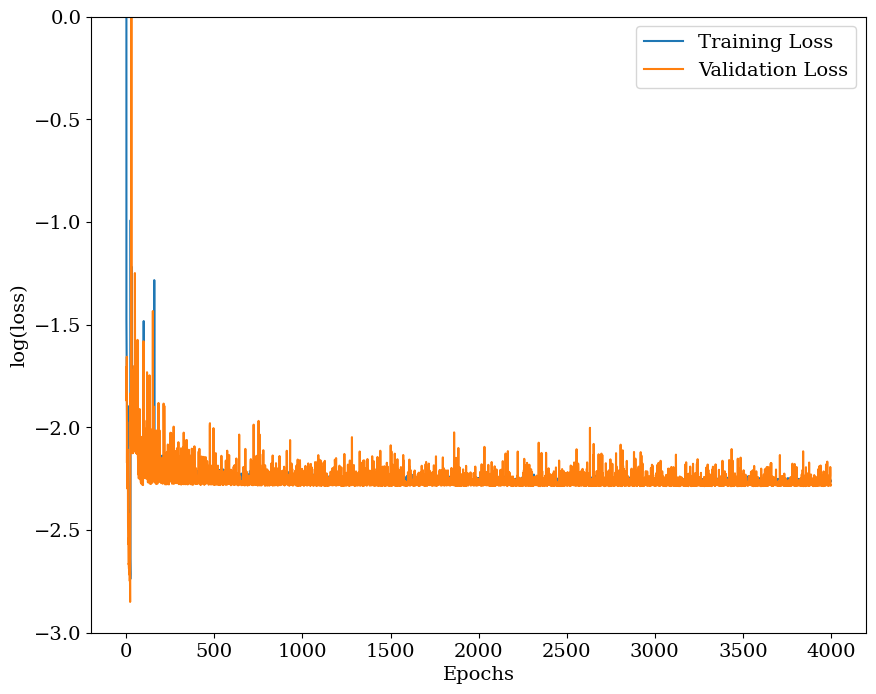
\includegraphics[width=\textwidth]{images/Chapter4/VGG16/vgg_history_full.png}
\caption{Full training history for VGG16 model.} 
\label{fig:vgg_history_a}
\end{subfigure}
\hspace{.6em}
\begin{subfigure}{.46\textwidth}
\centering
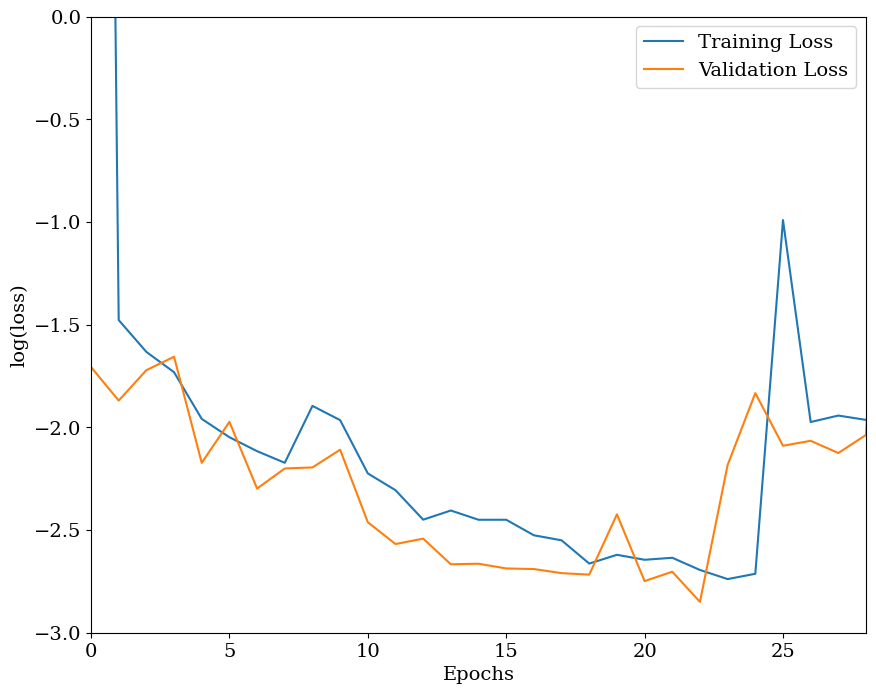
\includegraphics[width=\textwidth]{images/Chapter4/VGG16/vgg_history_zoom.png}
\caption{Zoom on the early dip.} 
\label{fig:vgg_history_b}
\end{subfigure}
\caption{Training history for the best performing VGG16 model. There is a dip very early after which the validation and training loss is considerable higher. In \autoref{fig:vgg_history_b}, a zoom on this dip is shown. The training loss is not developing at all after just a few epochs.}
\label{fig:vgg_history}
\end{figure}

Interestingly, the best performing VGG16 model started very strong by reducing the validation loss rapidly. For some reason tough, after around 25 epochs, the loss for both the validation and training set increased significantly and did not recover until the end of training. This shows that the model has difficulties finding anything useful in the provided images. Which is reflected in the bad predictions as well.

\begin{figure}[H]
\centering
\begin{subfigure}{.46\textwidth}
  \centering
  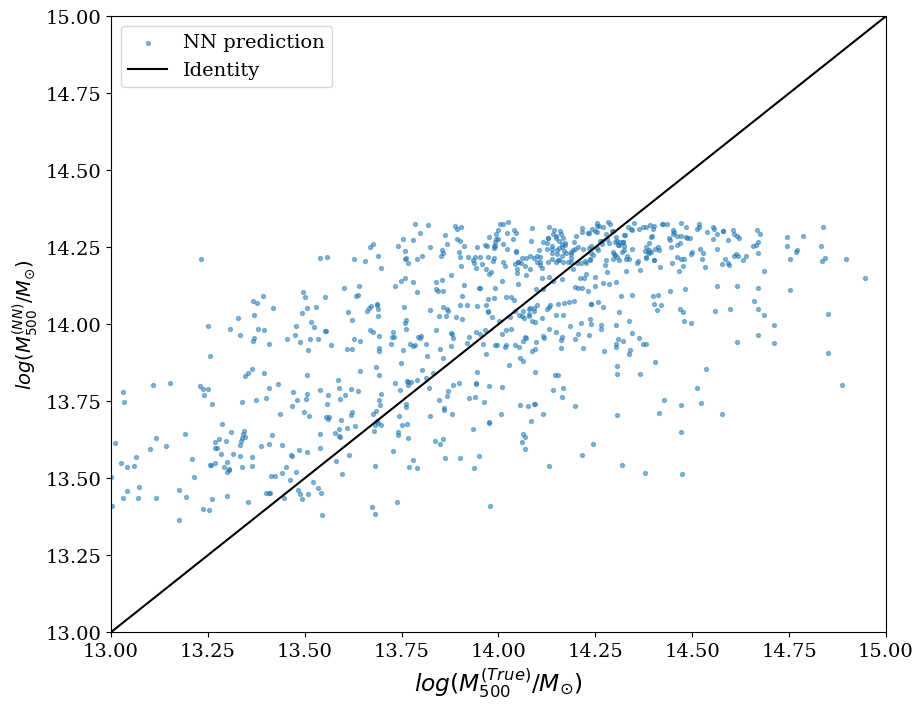
\includegraphics[width=\linewidth]{images/Chapter4/VGG16/vgg_pred_test.png}
  \caption{Model predictions on the test set.}
  \label{fig:best_perf_vgg16_a}
\end{subfigure}%
\hspace{.6em}
\begin{subfigure}{.46\textwidth}
  \centering
  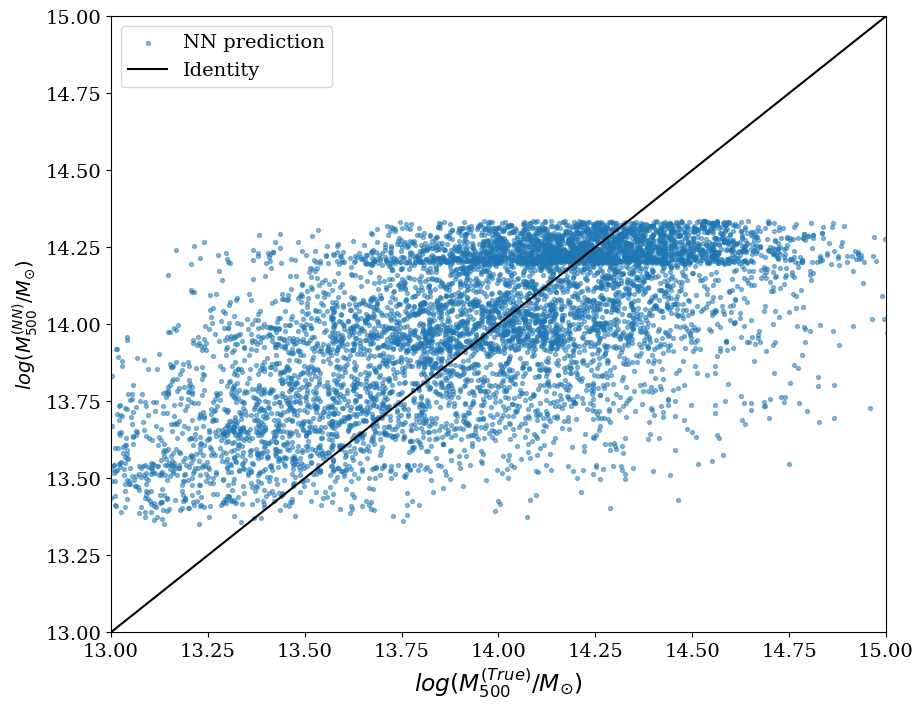
\includegraphics[width=\linewidth]{images/Chapter4/VGG16/vgg_pred_train.png}
  \caption{Model predictions on the training set.}
  \label{fig:best_perf_vgg16_b}
\end{subfigure}
\begin{subfigure}{.46\textwidth}
  \centering
  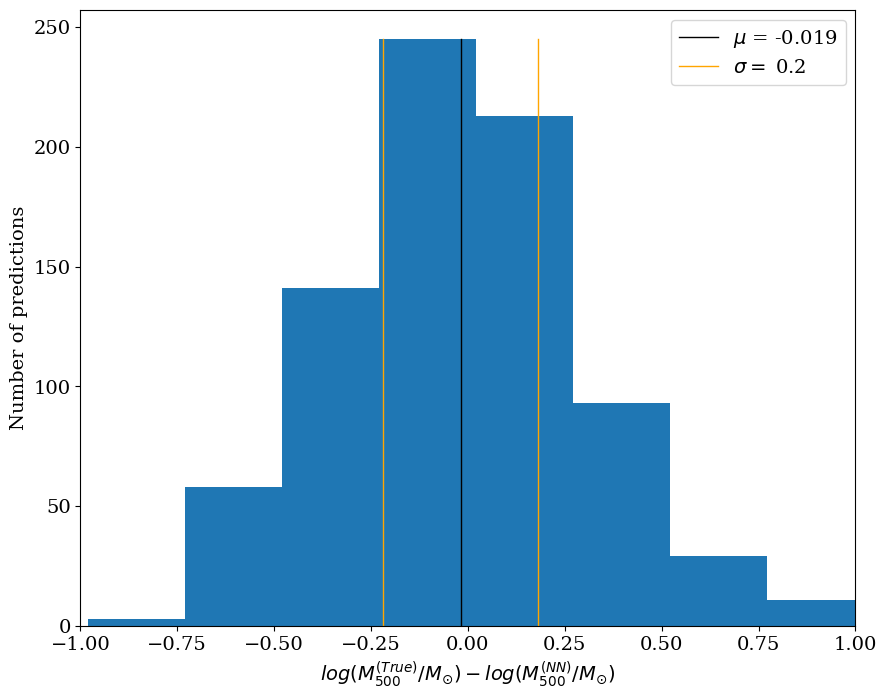
\includegraphics[width=\linewidth]{images/Chapter4/VGG16/vgg_pred_test_hist.png}
  \caption{Histogram of model predictions on the test set.}
  \label{fig:best_perf_vgg16_c}
\end{subfigure}%
\hspace{.6em}
\begin{subfigure}{.46\textwidth}
  \centering
  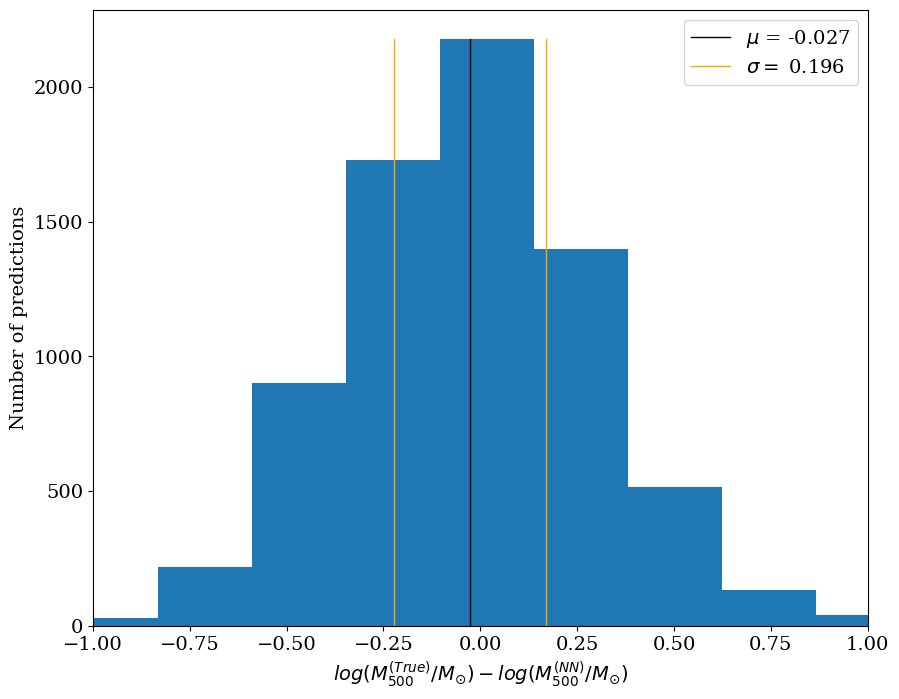
\includegraphics[width=\linewidth]{images/Chapter4/VGG16/vgg_pred_train_hist.png}
  \caption{Histogram of model predictions on the training set.}
  \label{fig:best_perf_vgg16_d}
\end{subfigure}
\caption{Prediction analysis for VGG16 model. This model struggled to achive good predictions. It did not predict any value above a mass of $\log{(M_{500}^{\text{true}}/M_{\odot})} \sim 14.4$. } 
\label{fig:best_perf_vgg16}
\end{figure}

The best model does not seem to overfit the training data. Nevertheless, the predictions are widely spread and there are even some horizontal lines visible within the predictions where the model seemed to predict a certain value for many different galaxy clusters (e.g. at masses around $\log{(M_{500}^{\text{true}}/M_{\odot})} = 13.9$ and $\log{(M_{500}^{\text{true}}/M_{\odot})} = 14.25$). I have seen this behaviour from all trained VGG16 models and do not yet understand the origin of this.